\section{Introduction}
\subsection{Problem Background}
The United States is experiencing an epidemic of drug overdose deaths. According to Centers for Disease Control (CDC), drug overdoses have dramatically increased over the last two decades, with deaths more than tripling between 1999 and 2016\footnote{See from Centers for Disease Control website, (\url{https://www.cdc.gov/features/confronting-opioids/index.html}), accessed 25 January 2019.}. In 2017, more than 72,000 Americans died from a drug overdose. At 197 people each day, this is more than the number of lives lost in car accidents or gun-related homicides, which is declared by U.S. DEPARTMENT OF AGRICULTURE\footnote{See from U.S. Department of Agriculture website, (\url{https://www.usda.gov/topics/opioids}), accessed 25 January 2019.}. An overwhelming majority of these overdose deaths involved opioids.

Opioids are a type of narcotic pain medication. And morphine, which is well known, is the most widely used opioid analgesic. In addition, opioids include fentanyl, codeine, methadone, etc. In addition to analgesia, opioids can also be used for cough, diarrhea, and sedation. In 2000, WHO proposed: "In all analgesic treatments, opioid analgesics are essential for the treatment of cancer pain. Especially for patients with moderate and severe cancer pain, opioid analgesics have an irreplaceable position."

However, they may cause serious side effects if used incorrectly. Using opioids frequently may cause both mental and physical dependence; once people are addicted, it would be difficult to treat. For people who have an opioid addiction, their problem often starts with a prescription. They compulsively seek out the pain medications, which usually leads to negative consequences in their personal lives or workplace. They might take someone else’s pills or buy them off the street, which is especially dangerous since those drugs are often laced with lethal amounts of fentanyl. In addition, recent studies have found that opioids may also cause other health problems, such as an increased risk of hepatitis C and HIV infection with the use of injectable opioids for private use. 

In the United States, opioid abuse has been around for a long time. As early as the 1980s, some scholars believed that opioids were not severely addictive, while most opioid manufacturers in U.S. also aggressively promoted their products, promising that opioids were not addictive. This has led to a surge in opioids. Furthermore, the huge opioid market in the United States may also be the motivation for many pharmaceutical companies to take risks. From the perspective of medical insurance expenses, addiction treatment, criminal justice investigation, etc., the United States suffers economic losses of up to 80 billion US dollars due to the abuse of opioids every year.

The United States has set up a drug control bureau, the U.S. Drug Enforcement Administration (DEA), to set corresponding production quotas for controlled substances such as opioids to meet the practical requirements of medical treatment, scientific research, export, and storage, etc. In August 2017, the United States officially listed opioids as “national emergency”.

Figure \textbf{\ref{ratesByState2016}} shows the number and age-adjusted rates of drug overdose by state in 2016 in the U.S. From the perspective of the problem requested, particularly, the five targeted states surrounded by blue contour lie in the district which suffered the drug overdose most severely, among which, comparatively speaking, Virginia was damaged the most slightly, from 13.6 to 16.0.
\begin{figure}
	\centering
	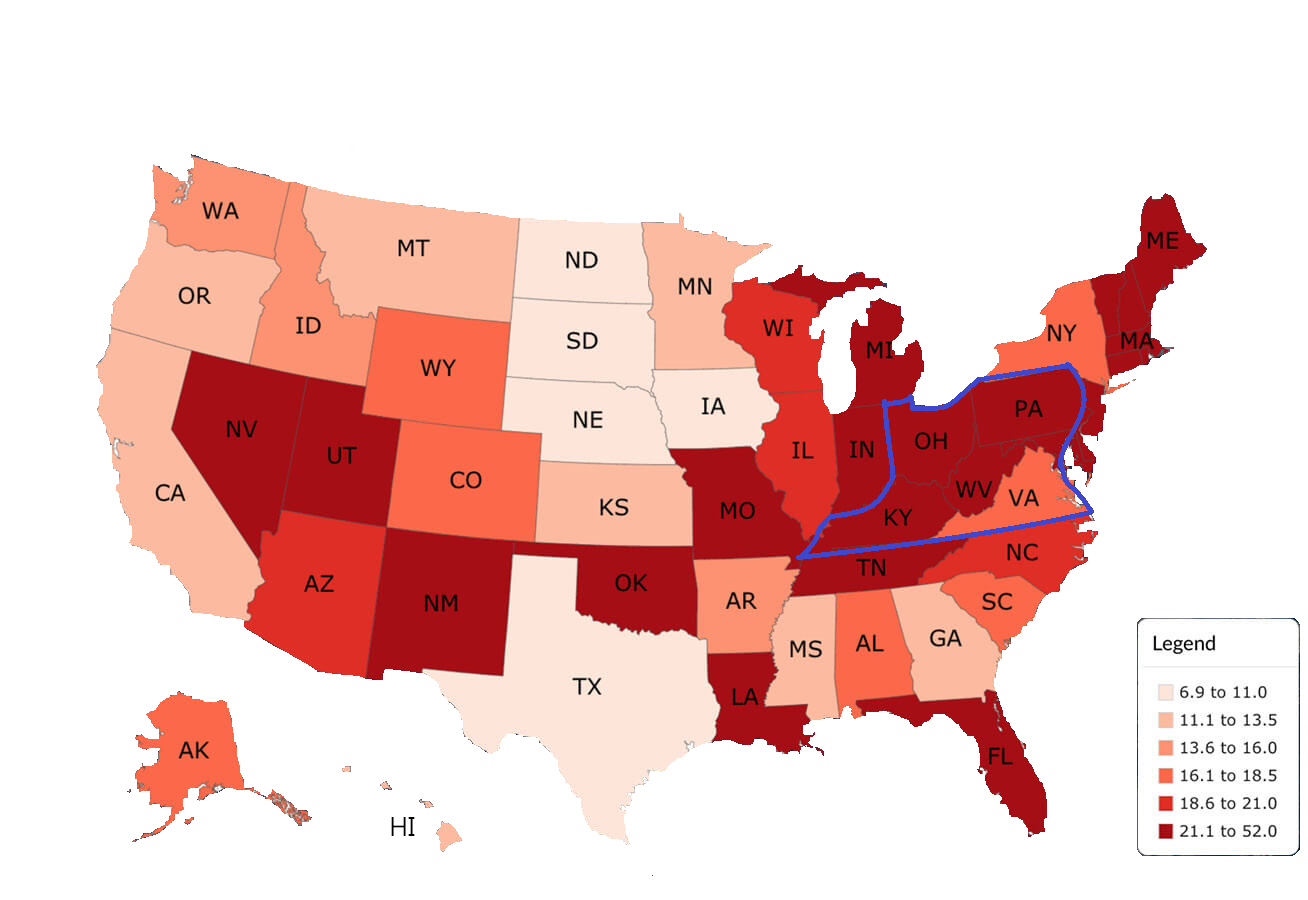
\includegraphics[scale=0.5]{ratesByState2016.png}
	\caption{Number and age-adjusted rates of drug overdose by state, US 2016.}
	\label{ratesByState2016}
\end{figure}

%Two major problems are discussed in this paper, which are:
%\begin{itemize}
%    \item Doing the first thing.
%    \item Doing the second thing.
%\end{itemize}

\subsection{Literature Review}
Researches about the opioid use are abundent, varying from the mathematical model establishment to the evaluation of social consequence, and also from the association with other diseases to the strengths for treatment.
Paper \cite{3} validates the feasibility of the epidemiologic method to the spread of heroin use, with particular emphasis on the analogy between heroin use and communicable disease. This inspires us to transfer the epidemic model for this problem.

Rather than use the epicdemic model, the authors \cite{5} designed Hierarchical Bayesian Poisson space–time analysis to relate the prescription opioid (PO) poisoning spread with spatial contagion and other social properties. In addition, the distribution of age-related and work-place-related sources of medical need for POs in rural area can partly explain the growth of PO poisoning.

From the pespective of consequence caused by it, authors of paper \cite{4} investigated the association of maximum prescribed daily opioid dose and dosing schedule with risk of opioid overdose death. They suggested that among patients receiving opioid prescriptions for pain, higher opioid doses were more associated with increased risk of opioid overdose death.

Considering the kinds of epidemic models, the author \cite{6} surveyed previous models for the spread of infectious diseases in populations with age structure, heterogeneity, and spatial structure. Similar results with new expressions for the basic reproduction number $R_0$ are obtained in his survey.

\subsection{Our work}
In this paper, we make a quantitative and qualitative analysis on the reported synthetic opioid and heroin incidents between these five states and their counties over time and identify some strategies for countering the opioid crisis.

We establish an SIS model to stimulate the spread of the drug incidents between and inside five states. This model derives from the epidemic model, which fits the spread characteristics of the opioid use.

Furthermore, we develop the solution to the inverse problems about differential equation parameters of the SIS model with the Genetic Algorithm \textbf{GA}, for the difficulty solving enormous dimension of the parameter matrix. This model enhances the robustness and the convergence of solution, yet at the cost of the accuracy and computation capacity. 

As for the first problem, we need to propose a mathematical model to fit the drug reports of five states, and to identify any possible places that might have started the opioid trends now. To solve these problems , we predict the trend of drug reports (take fentanyl as an example) by our model and divide the state into several blocks to narrow up the target places.

As for the second problem, we need to identify any possible factors from given socio-economy data that are associated with the opioids overdosing, as well as the specific degree of this relation. So we improve our model, considering these factors in it. And then, our model fits the real data better than before, with train error varying from $0.077$ to $0.045$.

As for the third problem, we need to produce a strategy that can solve the opioids crisis and identify its effectiveness by our model as well as the optimal boundaries of parameters. We analyze the parameter characteristics of our model, and then find the important impact of the flow of opioid use from other places on a state. We propose to pay more emphsis on it.
Finally, we analyze the sensitivity of our model.


\section{Preparation of the Models}
\subsection{Assumptions}
According to the paper [6], we set up the following assumptions for the SIS model.
\begin{enumerate}[\bfseries A.]
    \item The population N is constant in a fixed place, including states and counties. People are divided into two groups: Susceptible group and Infective one.
    \item The infectious ratio in and between two places ($i, j$) is considered as, take $j\rightarrow i$ as an example, $$\frac{a_{ij}I_{j}}{N_j}$$ where $a_{ij}$ is the weight that Place $j$ affects Place $i$, $I_j$ is the infective number in Place $j$.
    \item Define the average effective contact number of infective members in Place $i$ as $\lambda_i$, $$\lambda_i=\sum_{j=1}^n{\frac{a_{ij}I_j}{N_j}} $$ where $n$ is the number of places that have impact on Place $i$.
    \item Any state (or county) we know only affects those states (or counties) that are no more than 1 state (or county) away from it, no matter how small they are.
    \item The number of reports for both each possible factor and each sub-division of the factor is linearly distributed over time. This hypothesis is obtained by observing the characteristics of the data set.
    \item For the sake of simplicity, and considering the macro regulation of the government policies, we assume that the recovery rate in each place varies linearly over time.
    \item We assume that it’s reasonable to narrow down the range of parameters based on prior knowledge or experience, such as each state's self-impact is greater than that of other states on itself. This is because, compared with the number of parameters of the model, the size of given dataset samples is too small, which would result in an unsatisfactory fit in the absence of specific conditions.
    \item The number of drug reports in a state will not be affected by the economic conditions, marital status and other social factors in other states, but only affected by those factors in the state itself. This is an naturally acceptable hypothesis.
\end{enumerate}

\subsection{Notations}
The primary notations used in this paper are listed in \textbf{Table \ref{Ntt}}.
\begin{table}[h]
    \begin{center}
        \caption{Notations}
        \begin{tabular}{cl}
            \toprule
            \multicolumn{1}{m{2cm}}{\centering Symbol}
            &\multicolumn{1}{m{13cm}}
              {\centering Definition}\\
            \midrule
            $a_{ij}$&Effective contact ratio per patients in Place $j$ with people in Place $i$\\
            $A$&$\left\{ a_{ij} \right\} _{n\times n}$\\
            $I_i$ &Drug identification (Infective) number in Place $i$, $i=1, 2, 3, \cdots, n$\\
            $I$ &$\left( \begin{matrix}
	I_1&		I_2&		\cdots&		I_{n}\\
\end{matrix} \right) ^T$\\
			$n_c$ &Number of given counties\\
			$n_s$ &Number of given states\\
			$N_i$ &Total population in the Place $i$\\
			$I/N$ &Infective ratio in places at the same level: $\left( \begin{matrix}
	\frac{I_1}{N_1}&		\frac{I_2}{N_2}&		\begin{matrix}
	\cdots&		\frac{I_{n}}{N_{n}}\\
\end{matrix}\\
\end{matrix} \right) ^T$\\
			$S_i$ &Susceptible number in Place $i$\\
			$S$ &$\left( \begin{matrix}
	S_1&		S_2&		\cdots&		S_{n}\\
\end{matrix} \right) ^T$\\
			$\gamma_0^{i}$ &The constant coefficient of recovery rate of Place $i$\\
			$\gamma_1^{i}$ &The linear coefficient of recovery rate of Place $i$\\
			$\gamma_t^{i}$ &The recovery rate of Place $i$ in the year $t$, $\gamma_t^{i}=\gamma_0^{i}+\gamma_1^{i}t$\\
			$\varGamma$ &$\left( \begin{matrix}
	\gamma _{0}^{1}&		\gamma _{0}^{2}&		\cdots&		\gamma _{0}^{n}\\
	\gamma _{1}^{1}&		\gamma _{1}^{2}&		\cdots&		\gamma _{1}^{n}\\
\end{matrix} \right) ^T$\\
			$\lambda_i$ &Average effective contact number of infective members in Place $i$\\
			$\sigma_i$ &Average effective contact number of patients in Place $i$ in infective period\\
			$KY$&Kentucky\\
			$OH$&Ohio\\
			$PA$&Pennsylvania\\
			$WV$&West Virginia\\
			$VA$&Virginia\\
            \midrule
            \multicolumn{2}{m{15.2cm}}{\textit{Notes}: If the parameter is superscripted with $c$, it means the place is at the level of counties; if it is superscripted with $s$, it means the place is at the level of states. Otherwise, it is considered to be at a comprehensive level.}\\
            \bottomrule
        \end{tabular}\label{Ntt}
    \end{center}
\end{table}

\section{The Models}

\subsection{Model 1: SIS Model}
\subsubsection{Detail about Model 1}
Due to the spread of the synthetic opioids and heroine incidents among states, we take the factor of impacts from other locations into consideration when setting the equation of the SIS model. Paper \cite{6} has indicated the feasibility of applying epidemic model to the spread of heroine utility; therefore, we determine to apply SIS model which fits the practical situation of drug spread.

In specific, we can get the following differential equation array:
\begin{eqnarray}
\begin{aligned}\label{arrayy_diff}
	\frac{\text{d}S_i}{\text{d}t}&=-\sum_{j=1}^n{\frac{a_{ij}I_j}{N_j}S_i}+\gamma _iI_i\\
	\frac{\text{d}I_i}{\text{d}t}&=-\frac{\text{d}S_i}{\text{d}t}\\
\end{aligned}\left( i=\text{1,2,}\cdots ,n \right)
\end{eqnarray}

%We can transform these $n$ equation arrays into a concise matrix form:
%\begin{eqnarray}\label{array_diff}
%\begin{aligned}
%	\frac{\text{d}S}{\text{d}t}&=-\text{diag}\left( S %\right) A\left( I/N \right) +\text{diag}\left( I \right) \varGamma\\
%	\frac{\text{d}I}{\text{d}t}&=-\frac{\text{d}S}%{\text{d}t}
%\end{aligned}
%\end{eqnarray}

%where $\text{diag}\left( S \right)\triangleq\text{diag}\left(S_1,S_2,\cdots ,S_n\right)$,$\text{diag}\left( I \right)\triangleq\text{diag}\left(I_1,I_2,\cdots ,I_n\right)$.

%In the equation (\ref{array_diff}), parameter matrixes $A$ and $\varGamma$ are unknown, while other parameters are given in the EXCEL attachment.

We first experiment the traditional approach to solving the differential equations. That is, we apply the trust region method \cite{7} for the inverse problem about differential equation parameters. According to the algorithm introduced in paper \cite{7}, we transform the problem into a minimization problem, the objective function of which is as following:
\begin{equation}\label{objective}
f\left( A,\gamma _1,\gamma _2,\cdots ,\gamma _n \right) =\frac{1}{ns}\sum_{i=1}^n{\sum_{t=0}^s\left[\frac{\widehat{I}_{i,t}\left( A,\gamma _1,\gamma _2,\cdots ,\gamma _n \right) -I_{i,t}}{I_{i,t}}\right]^2}
\end{equation}
where $A,\gamma_1, \gamma_2,\cdots , \gamma_m$ are parameters, $\widehat{I}_{i,t}\left( A,\gamma _1,\gamma _2,\cdots ,\gamma _m \right) $ is the corresponding predicted value of $I_i$ in the year $t$ ($t=0,1,\cdots,s$) after $A, \gamma_1, \gamma_2, \cdots , \gamma_m$ are obtained, and $I_{i,t} $ is the practical value $I_i$ in the year $t$ ($t=0,1,\cdots,s$).

\begin{equation}
\begin{aligned}\label{min}
&\min\text{ }\varphi _i\left( a_{i1},a_{i2},\cdots ,a_{in},\gamma _i \right)\\
=&f_i\left( \left( a_{i1}^{\left( k \right)},a_{i2}^{\left( k \right)},\cdots ,a_{in}^{\left( k \right)},\gamma _{i}^{\left( k \right)} \right) \right)+  
\\
&\nabla f_i\left( \left( a_{i1}^{\left( k \right)},a_{i2}^{\left( k \right)},\cdots ,a_{in}^{\left( k \right)},\gamma _{i}^{\left( k \right)} \right) \right) ^T\left( a_{i1},a_{i2},\cdots ,a_{in},\gamma _i \right)+ 
\\
&\frac{1}{2}\left( a_{i1},a_{i2},\cdots ,a_{in},\gamma _i \right) ^T\nabla ^2f_i\left( \left( a_{i1}^{\left( k \right)},a_{i2}^{\left( k \right)},\cdots ,a_{in}^{\left( k \right)},\gamma _{i}^{\left( k \right)} \right) \right) \left( a_{i1},a_{i2},\cdots ,a_{in},\gamma _i \right)
\end{aligned}
\end{equation}
where $\lVert a_{i1},a_{i2},\cdots ,a_{in},\gamma _i \rVert \leqslant r_k, i=\text{1,2,}\cdots ,n$.

To program this algorithm, we compute the $Hessian$ matrix of points in the trust region. And then substitute the $Hessian$ matrix, along with the gradient matrix, into equation $\left(\ref{min}\right)$ to find out the point corresponding to the minimum value, which should be the optimal solution currently. Thirdly, re-divide the trust region according to different conditions of the optimal solution, and iterate above steps until the gradient of the point is lower than the threshold so that we obtain the final optimal solution.

However, the weakness of this algorithm is the high complexity for computation. As is known, the $Hessian$ matrix is at the dimension of $n^2\times n^2$ for $n$ parameters, which will cause a heavy burden to the computation with the increase of $n$. What’s more, both the gradient matrix and the $Hessian$ matrix are time-consuming to conduct, thus being impossible to for us to solve the inverse problems at the level of counties particularly.

Therefore, we decide to develop the approach to solving this model in an attempt to decrease the complexity when facing the enormous data to be computed. Specifically, we apply the $GA$ model to search the solution to parameters.

For the part 1 problem, we choose the following function as the objective function.
\begin{equation}
\min\text{ }f\left( A^s,\gamma _{1}^{s},\gamma _{2}^{s},\cdots ,\gamma _{n_s}^{s} \right) =\frac{1}{n_ss}\sum_{i=1}^{n_s}{\sum_{t=0}^s{\left| \frac{\widehat{I}_{i,t}^{s}\left( A^s,\gamma _{1}^{s},\gamma _{2}^{s},\cdots ,\gamma _{n_s}^{s} \right) -I_{i,t}^{s}}{I_{i,t}^{s}} \right|}}
\end{equation}

This is one at the level of states, which, with the help of the GA model, can offer us the convergent solution to parameters. The result of the parameter matrix is given below.
\begin{equation}
A=\left[ \begin{matrix}
	0.50713517&		0.02263958&		0.07114156&		0.40748377&		0.24293688\\
	0.00092936&		0.64209954&		0.16669959&		0.17898226&		0.14229662\\
	0.00250955&		0.24609878&		0.50347999&		0.02277512&		0.20417946\\
	0.01678149&		0.0914572&		0.01279008&		0.68407223&		0.06001597\\
	0.00268578&		0&		0.01794575&		0.00094326&		0.78687606\\
\end{matrix} \right] 
\end{equation}
\begin{equation}
\varGamma =\left[ \begin{matrix}
	0.86816492&		0.99901323&		0.9356767&		0.96664902&		0.6449881\\
	0.02645234&		-0.05330094&		0.07823487&		0.0726793&		0.06921307\\
\end{matrix} \right] 
\end{equation}
where index $i$ refers: $1\rightarrow KY, 2\rightarrow OH, 3\rightarrow PA, 4\rightarrow VA, 5\rightarrow WV$. We transfer the spread characteristics into the map (See Fig. \ref{SpreadLine}) so that we can have a clear view on it.
\begin{figure}
	\centering
	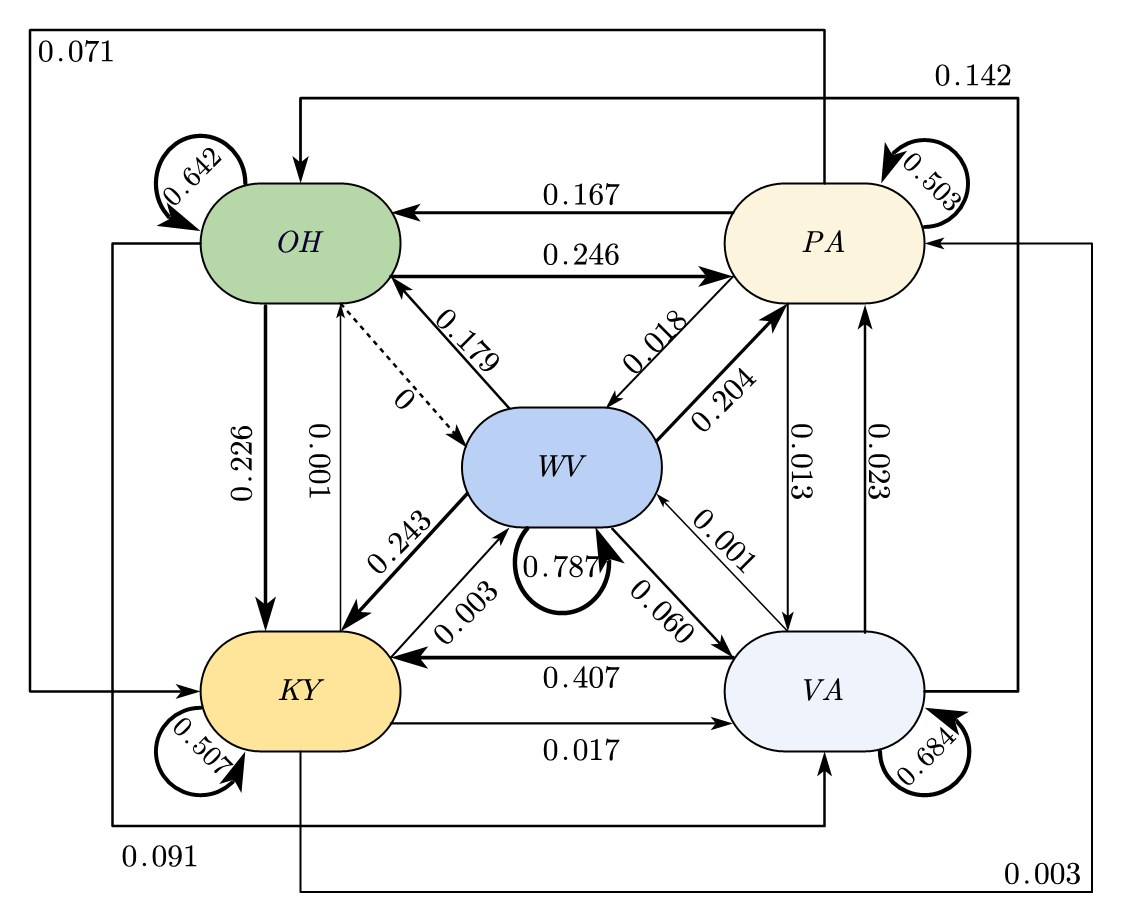
\includegraphics[scale=0.45]{SpreadLine.png}
	\caption{Map of five states and Weight of Spread Lines.}
	\label{SpreadLine}
\end{figure}

We implement the modeled parameters into the equation \ref{arrayy_diff} or \ref{array_diff}, getting the predicted situation of specific drug reports in five states respectively. The comparation between the real reports and predicted reports is showed in the Fig. \ref{drug_five}. We can find that our model fits the real situation well. The training error is $0.077$ for our model.

\begin{figure}[htbp]
\centering
\subfigure[KY]{
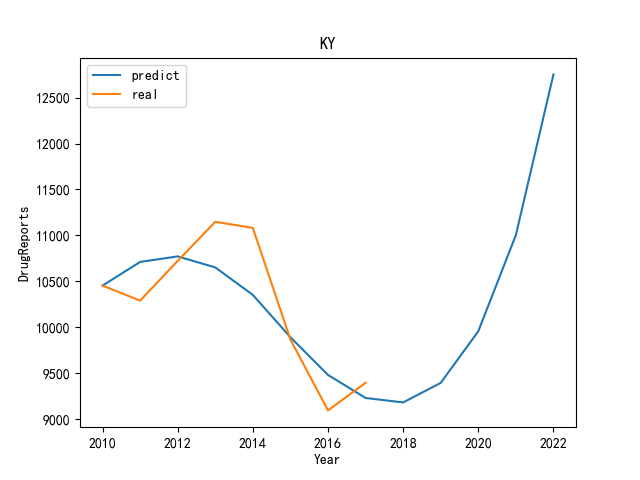
\includegraphics[scale=0.43]{KY.png}
}
\quad
\subfigure[OH]{
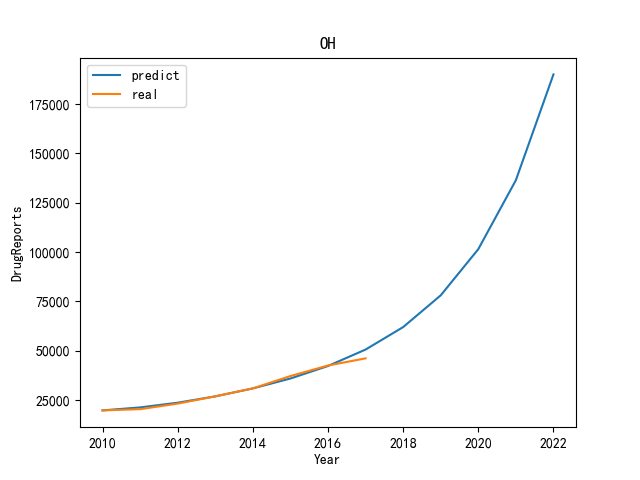
\includegraphics[scale=0.43]{OH.png}
}
\quad
\subfigure[PA]{
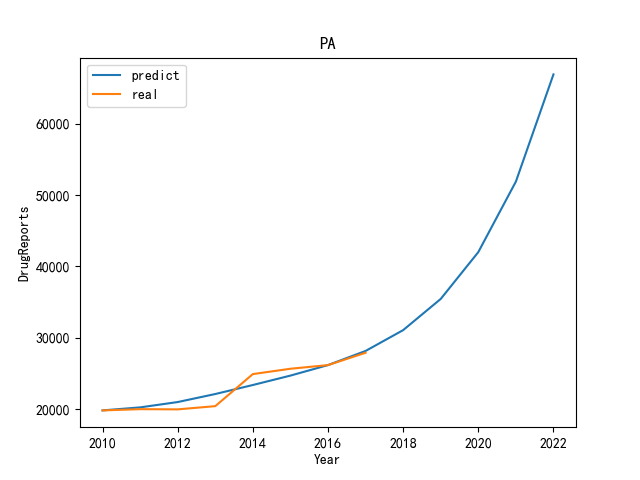
\includegraphics[scale=0.43]{PA.png}
}
\quad
\subfigure[WV]{
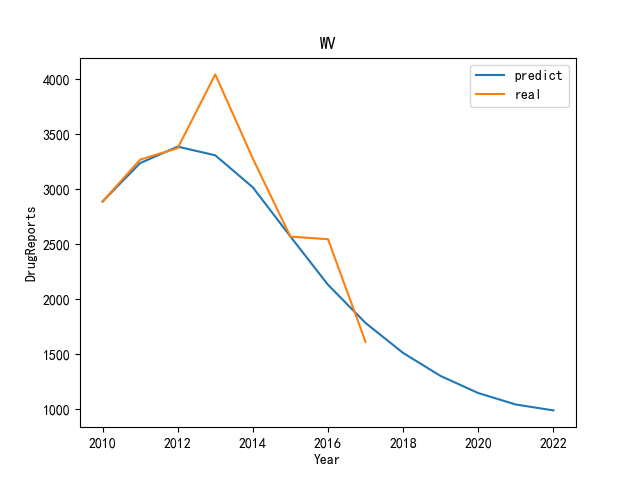
\includegraphics[scale=0.43]{WV.png}
}
\quad
\subfigure[VA]{
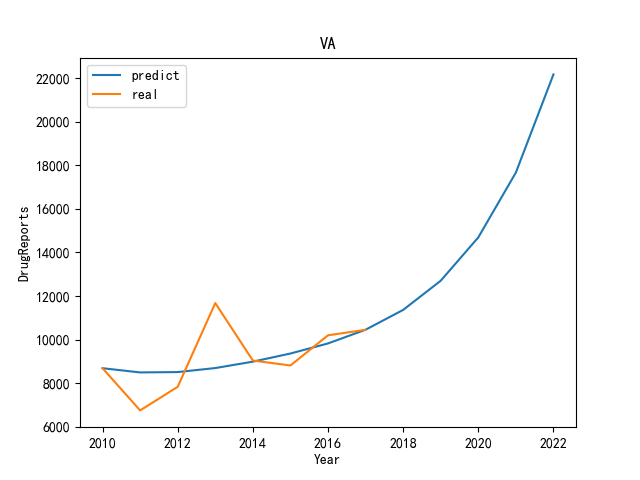
\includegraphics[scale=0.43]{VA.png}
}
\caption{The drug reports in five states.}\label{drug_five}
\end{figure}

%\begin{table}[h]
%    \begin{center}
%        \caption{usage}
%        \begin{tabular}{clcl}
%            \toprule
%           \multicolumn{1}{m{3cm}}{\centering Symbol}&\multicolumn{1}{m{3cm}}{\centering Definition}&\multicolumn{1}{m{3cm}}{\centering Data}\\
%            \midrule
%            $A$&the first one&\\
%            $b$&the second one&\\
%            $\alpha$ &the last one&\\
%            $\beta_t$ &the last last one&\\
%            \midrule
%            \multicolumn{1}{m{3cm}}{\centering Symbol}&\multicolumn{1}{m{3cm}}{\centering Definition}&\multicolumn{1}{m{3cm}}{\centering Data}\\
%            \bottomrule
%        \end{tabular}\label{N}
%    \end{center}
%\end{table}

\paragraph{Analysis}
From the perspective of the epidemic model, namely SIS model, we can get the relation between the $\sigma_i$ and $\lambda_i , \gamma_i$. That is $\sigma _i=\lambda _i/\gamma _i$ . Then from the article \cite{8}, we can learn the different change trend in the different extent of $\sigma$. To be specific, the trend goes like the Fig. \ref{SIS_sigma}. We can get the conclusion that the trend in five states can match the part of the curves in Fig. \ref{SIS_sigma} respectively. For example, the predicted line of OH corresponds to the situation that $\frac{I\left( 0 \right)}{N}<1-\frac{1}{\sigma}$ and $\sigma>1$, while that of WV is more likely to match the situation that $ \sigma \leqslant 1$. This suggest that our model can fit the synthetic opioids crisis well in these five states.
\begin{figure}
	\centering
	
\includegraphics[scale=0.5]{SIS_sigma.png}
	\caption{$\frac{I}{N}$\text{-}$t$ figures in SIS.}
	\label{SIS_sigma}
\end{figure}

Next, we propose a further study on a specific opioid: fentanyl. Fentanyl has been an issue that can not be ignored in recent years. The number of fentanyl drug reports from 2010 to 2017 is projected on a county-scale map as shown in Fig. \ref{FentylReports2}.

The figure indicates that state OH is sufferring from a severe fentanyl crisis. Therefore it is necessary to model the fentanyl spread and characteristics of OH, and then find the proper drug identification threshold levels to contain the crisis. However, fitting all the counties of OH separately into the model is not feasible as a huge amount of computational resources will be needed. Therefore, we choose to divide the whole OH state into six large blocks and put them into the model for prediction. The way of dividing is shown in Fig. \ref{OH_DIVIDE}.
\begin{figure}
	\centering
	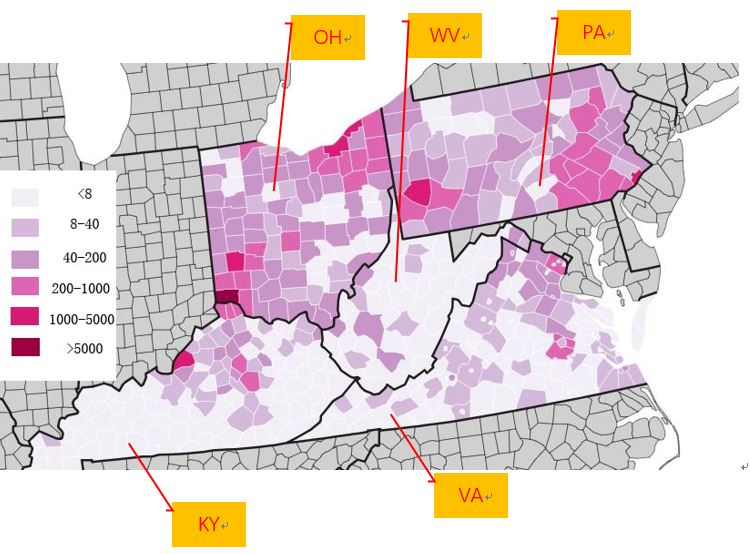
\includegraphics[scale=1.2]{FentylReports2.jpg}
	\caption{Fentyl reports number of all the counties in five states.}
	\label{FentylReports2}
\end{figure}
\begin{figure}
	\centering
	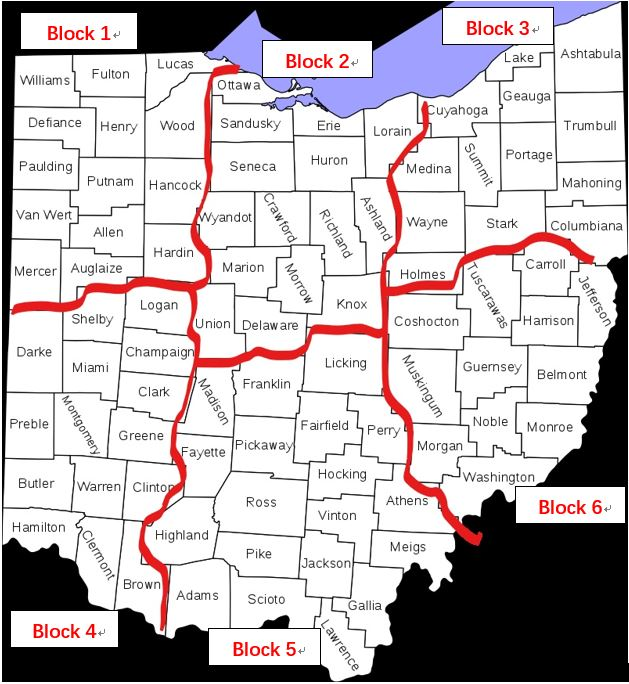
\includegraphics[scale=0.9]{OH.jpg}
	\caption{The way of dividing State OH into six parts.}
	\label{OH_DIVIDE}
\end{figure}

After obtaining the model parameters between the six blocks, we predict their trend in the next few years. According to result showed in the Fig. \ref{no_action} with blocks 3 and 4 rising at the fastest rate, indicating that the two regions are likely to explode in the next few years.
\begin{figure}
	\centering
	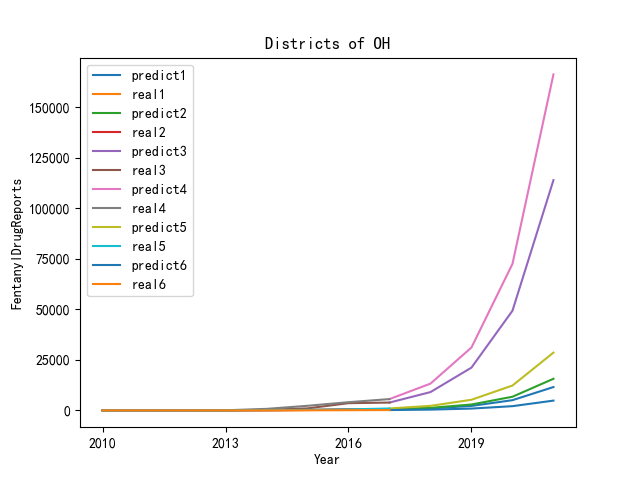
\includegraphics[scale=0.6]{no_action.png}
	\caption{The trend of fentanyl reports of six parts.}
	\label{no_action}
\end{figure}

If the patterns and characteristics continue, i.e. the $\gamma_0$,$\gamma_1$,$A$ parameters of the model remain unchanged, the number of fentanyl drug reports in the 3rd and 4th block is expected to have a sharp increase at around 2019 (Fig. \ref{OH_DIVIDE}). The U.S. government should draw enough attention to prevent the incident from happening.

To identify the location and the time that might have started in these five states, we hold the view that where there is a growing trend of specific drug reports in the next few years, there might have been the start of this drug reports. And regarding to the threshold of the occurrence, we think that the higher the recovery rate in a state is, the more possible the drug reports cases will be to decrease in the next few years. As a result, we consider the threshold of the recovery rate, namely $\gamma_i$ in each state, as the threshold of the occurrence, which means searching the maximum value of $\gamma_i$ that makes the reports number increase in the next few years.

Fig. \ref{gamma_0} represents 12 predictions with different drug identification threshhold levels taken after 2017. The threshhold level is represented by the $\gamma_0$,$\gamma_1$ parameters of the model. Hard threshholds can be decribed by large value of $\gamma_0$,$\gamma_1$ while soft threshholds can be described by small ones. When the drug identification threshhold is softer than that of $(\gamma_0$,$\gamma_1)=(0.9,0)$ or $(0.8,0.05)$ or $(0.7,0.1)$, the incident is likely to occur at around 2021, in the 3rd and 4th block of State OH.
\begin{figure}[h]
	\centering
	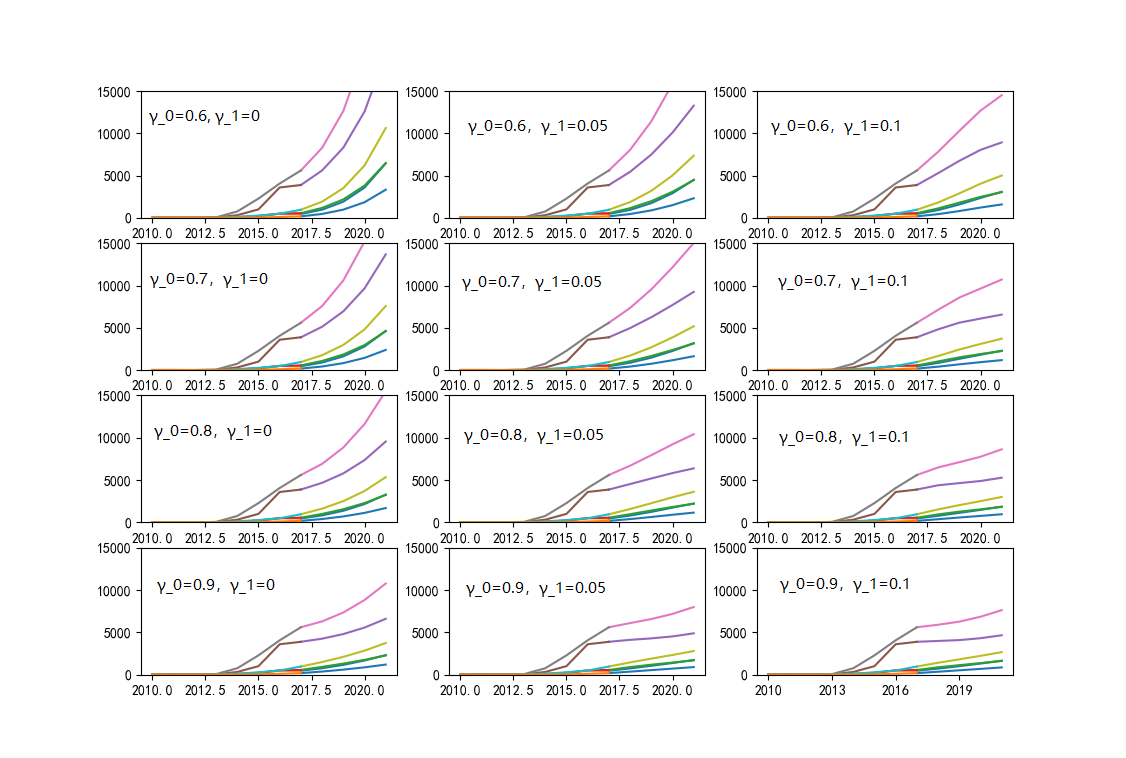
\includegraphics[scale=0.6]{gamma_0.png}
	\caption{The trend of fentanyl reports of six parts.}
	\label{gamma_0}
\end{figure}

\subsection{Model 2: Developed SIS Model}
\subsubsection{Detail about Model 2}
Concerning the good number of factors that we do not take into consider but do have contribution to the drug report trend, we choose to improve our model. That is to add the weight of those possible factors into the model. By training the parameter matrix, we can finally research the correlation between the factors and the drug reports in each states. To be specific, we can get the following differential function array:
\begin{eqnarray}
\begin{aligned}
&\frac{\text{d}S_i}{\text{d}t}=-\left( \sum_{j=1}^n{\frac{a_{ij}I_j}{N_j}} \right) \exp \left( \frac{1}{\sum_{\iota =1}^L{K_{\iota}}}\sum_{\iota =1}^L{\sum_{\kappa =1}^{K_{\iota}}{\frac{\widehat{\beta _{0}^{\kappa \iota}}+\widehat{\beta _{1}^{\kappa \iota}}t}{\widehat{\beta _{0}^{\iota}}+\widehat{\beta _{1}^{\iota}}t}}\rho _{i\kappa \iota}} \right) S_i+\left( \gamma _{0}^{i}+\gamma _{1}^{i}t \right) I_i
\\
&\frac{\text{d}I_i}{\text{d}t}=-\frac{\text{d}S_i}{\text{d}t}
\end{aligned}\label{modifyfunction}
\end{eqnarray}

where the parameter:
\begin{itemize}
	\item $L$ is the number of the factors selected from given data;
	\item $K_\iota$ is the number of the subdivision of factor $\iota$;
	\item $\widehat{\beta _{0}^{\kappa \iota}}$ is the constant coefficient of the linear regression of the kth sub-factor of factor $\iota$.
	\item $\widehat{\beta _{1}^{\kappa \iota}}$ is the linear coefficient of the linear regression of the kth sub-factor of factor $\iota$.\\
	\item $\frac{\widehat{\beta _{0}^{\kappa \iota}}+\widehat{\beta _{1}^{\kappa \iota}}t}{\widehat{\beta _{0}^{\iota}}+\widehat{\beta _{1}^{\iota}}t}$ is the ratio of the fitted sub-division portion of factor $\iota$.\\
	\item $\rho$ is the weight of the correlation between the factor and the local drug reports number.
\end{itemize}

In this model, we establish a statistic in the form of $$\exp \left( \frac{1}{\sum_{\iota =1}^L{K_{\iota}}}\sum_{\iota =1}^L{\sum_{\kappa =1}^{K_{\iota}}{\frac{\widehat{\beta _{0}^{\kappa \iota}}+\widehat{\beta _{1}^{\kappa \iota}}t}{\widehat{\beta _{0}^{\iota}}+\widehat{\beta _{1}^{\iota}}t}}\rho _{i\kappa \iota}} \right)$$ to evaluate the performance of factors in improving the model. Firstly, utilizing the exponential function is in an attempt to magnify those significant drug reports, so that it can perform well in evaluating the degree of significance. On the other hand, we sum up the weight value of all possible factors (here we select three elements- education degree, disability, marital condition) for the fact that this method fits the dataset better than other models we have tried and have a good performance in improving the training error of our model. 

Our objective function is the same as the equation \ref{objective}. In this train procedure, we substitute the weight parameter $A$ and the coefficient matrix of recovery rate $\varGamma$ obtained from the model 1 into the equation \ref{modifyfunction}. The parameter to be optimized is $\rho_{i\kappa\iota}$. 

By training the processed data, then we get the result of the parameter matrix. It is showed in the Table. \ref{rho}. And the train error reduces to $0.045$, which performs better than model 1 ($0.077$). And the predicted curves of five states are showed in the Fig. \ref{drug_five_modify}
\begin{figure}
	\centering
	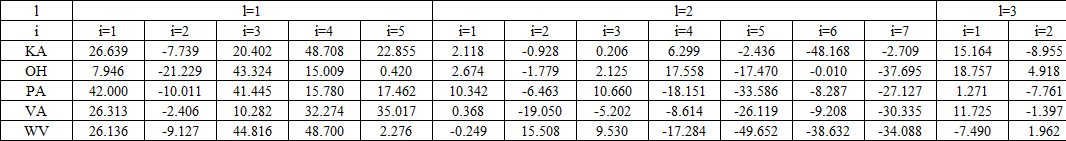
\includegraphics[scale=0.55]{rho.png}
	\caption{The matrix of $\rho_{i\kappa\iota}$, $\iota=1$ corresponds to marital conition, $\iota=2$ corresponds to educational degree,$\iota=3$ corresponds to disable or not. As for the meanings of index $i$ in each situation, see Table \ref{regression_coefficient}.}
	\label{rho}
\end{figure}

\begin{figure}[htbp]
\centering
\subfigure[KY]{
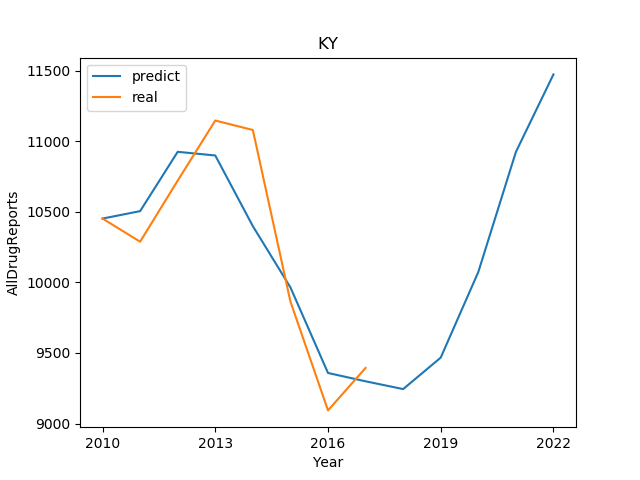
\includegraphics[scale=0.43]{KY_2.png}
}
\quad
\subfigure[OH]{
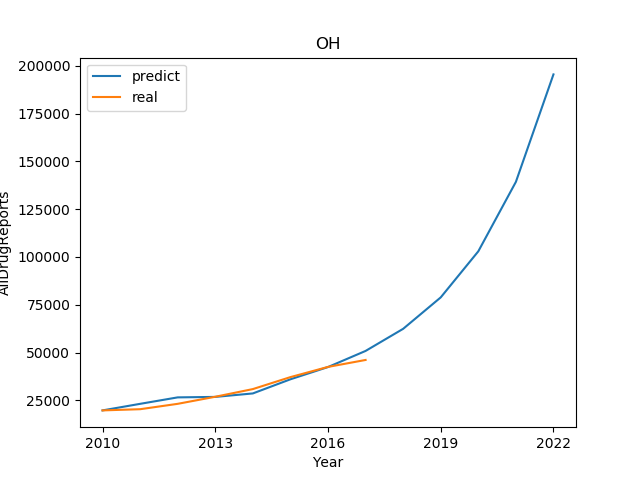
\includegraphics[scale=0.43]{OH_2.png}
}
\quad
\subfigure[PA]{
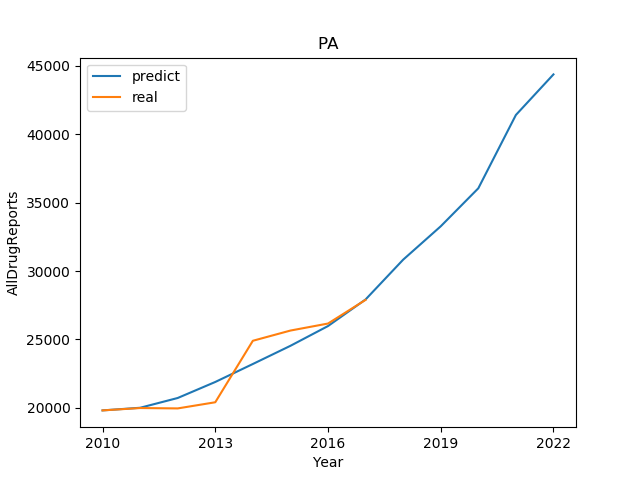
\includegraphics[scale=0.43]{PA_2.png}
}
\quad
\subfigure[WV]{
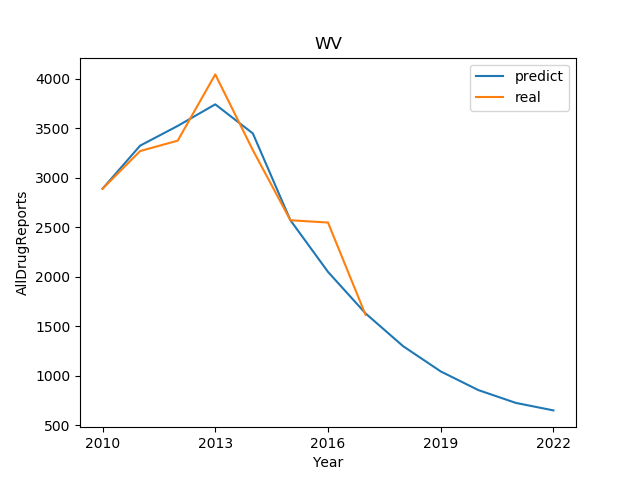
\includegraphics[scale=0.43]{WV_2.png}
}
\quad
\subfigure[VA]{
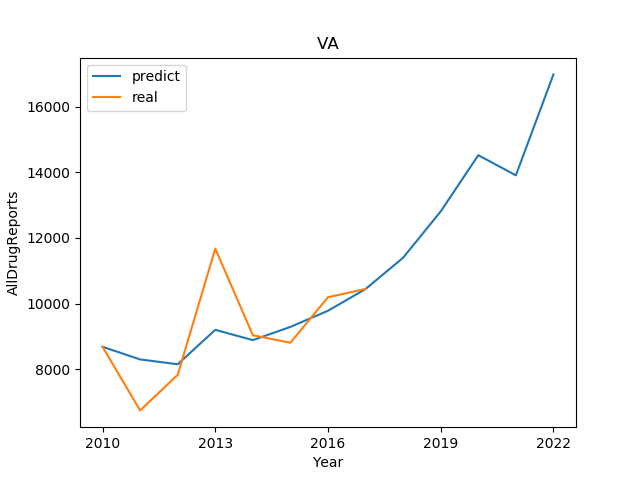
\includegraphics[scale=0.43]{VA_2.png}
}
\caption{The drug reports with modified model in five states.}\label{drug_five_modify}
\end{figure}

\subsubsection{Analysis}
From the table \ref{rho}, we can get several conclusions:
\subparagraph{$\iota=1$ (Marital Condition):} The poor marital condition has more correlation with the trends-in-use of opioids. In particular, those who live separated or widowed are more likely to use opioids in their life. This is mainly due to their seeking for things that can relieve them from their frustration in marriage.
\subparagraph{$\iota=2$ (Educational Degree):} The high educational degree can effectively decrease the risk of using opioids, which can be obtained by its significantly negative value.
\subparagraph{$\iota=3$ (Disable or not ):} Except from the value of WV, we can find that disability is also an important factor that has an impact on the trends-in-use of opioids. Some prescription drugs should be responsible for this factor because many of them like antalgic contain synthetic opioids that can cause patients to be tolerant with opioids if they take them over a long time. On the other hand, there is no significant relation between a health body and a low use of opioids.


Finally, combining the results from both model 1 and model 2, we can get the conclusion that the combination of the spread of use from other states and the socio-economy condition in the state when modelling the opioid incidents can represent the main characteristic of the progress of the opioid cases in and between these five states. As for the external factors, people across the borders, along with the potentially large requirements for prescription drugs from other places, are more associated with the spread of the opioids use, while as for the internal factors, besides the high possibility to access opioids users for the dense flow, many macro regulations are key to the future of such trends-in-use; for example, the development of local education to acknowledge the damage of such crisis, the access level to health care, the happiness level of local people and so on. Such statistical results indicate different problems that five states are facing according to our model results.

\subsubsection{Strategy for Crisis}
According to the results we predict, if we should devise a strategy that countering the opioid crisis, we would suggest that the spread of the opioids uses should be the main concern for these five states, because when we consider the internal factors, we find that the recovery rate of each state is commonly high, which means a coming decrease if the governments control the flow of opioid across the borders. In fact, the gamma coefficients of other states have increased with time, and only the gamma coefficient of OH state has become smaller and smaller with time. This may be because fentanyl has been popular in OH in recent years, and OH has not had time to do good countermeasures.

Therefore, it is imperative that OH State take effective measures against the fentanyl crisis and increase its own gamma coefficient to above $0.75$. Other states should ensure that their gamma coefficient does not decrease. On the other hand, the government should restrict the spread of drugs between states, reducing the non-diagonal elements of the A matrix to less than $80\%$ of the original value.The predicted results after the strategy implementation are shown in Fig. \ref{drug_five_strategy}.

The results suggest the effectiveness of our strategy. The increase rate of opioid report in State OH plunges to nearly zero in the coming years after the improvement of its recovery rate. And for other states, after we reduce the portion of opioid use from other states, for the high recovery rate, their drug reports plunge into a micro number comparative to their past data.
\begin{figure}[htbp]
\centering
\subfigure[KY]{
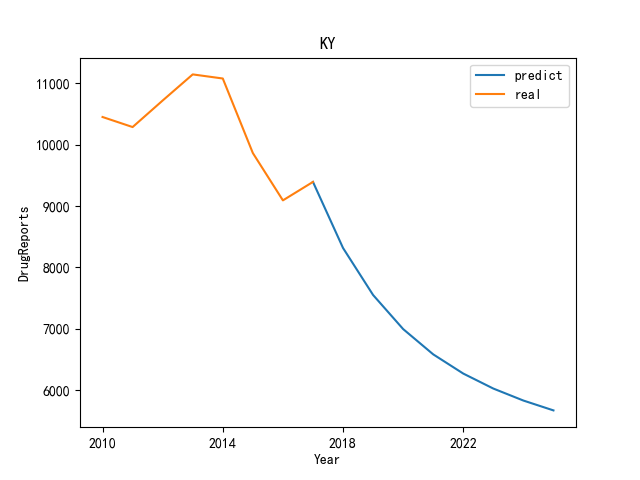
\includegraphics[scale=0.43]{KY_3.png}
}
\quad
\subfigure[OH]{
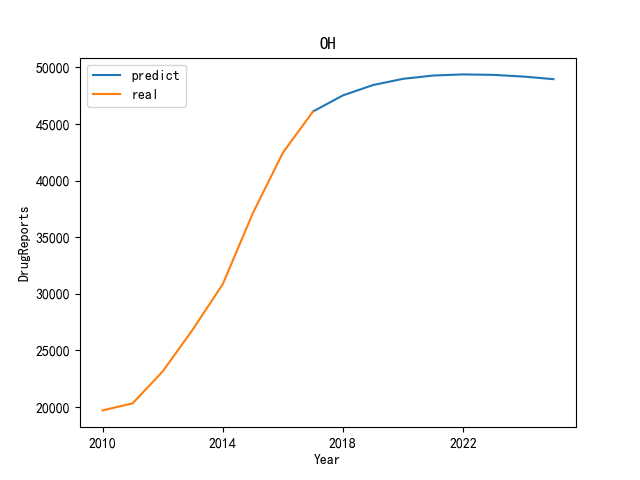
\includegraphics[scale=0.43]{OH_3.png}
}
\quad
\subfigure[PA]{
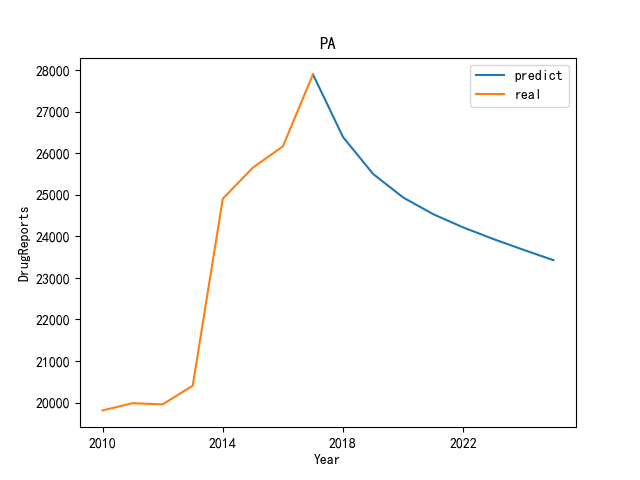
\includegraphics[scale=0.43]{PA_3.png}
}
\quad
\subfigure[WV]{
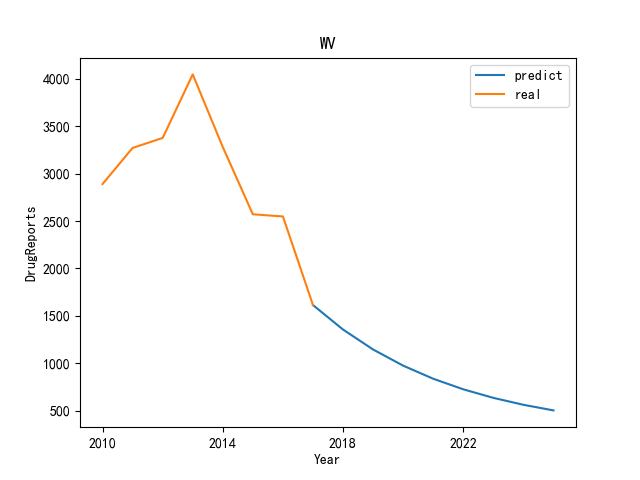
\includegraphics[scale=0.43]{WV_3.png}
}
\quad
\subfigure[VA]{
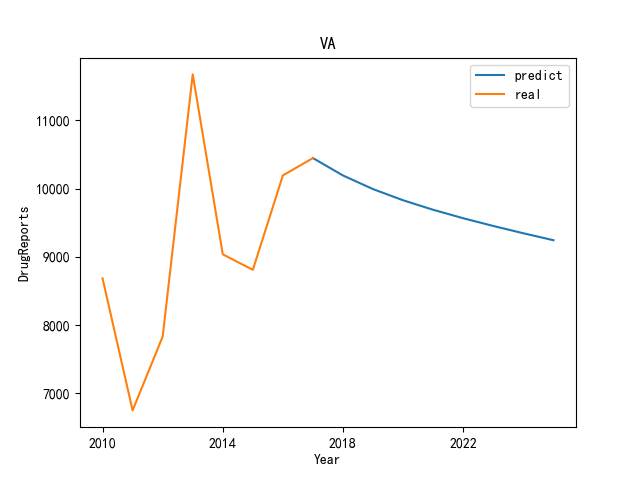
\includegraphics[scale=0.43]{VA_3.png}
}
\caption{The drug reports in five states after implementing the strategy.}\label{drug_five_strategy}
\end{figure}

\section{Conclusions and Discussion}
\paragraph{Conclusions:}
This paper manages to develop a fully data-based model to produce a regulation strategy for countering the opioid crisis. Our model exhibits a great potential in drawing the following conclusions:
\begin{itemize}
	\item We formulate a performance matrix for drug spread in and between five given states with the GA algorithm and improve the classic SIS model by considering the spread correlation of infection with other places and the dynamic characteristics of recovery rate.
	\item We identify three main performance contributing variables that generate a significant impact on the performance of the trends-in-use of opioids with the estimation of matrix $\rho$.
	\item We manage to devise a more practical epidemic model that predicts the system under the consideration of both inland and outland characteristics.
\end{itemize}

\paragraph{Limitation and discussion:}
Though our model successfully identifies the characteristic of the opioid crisis in five specific states, it can be improved from the following several respects:
\begin{itemize}
	\item As for the model 1, the performance of its prediction is affected by the number of total drug reports. This is due to the limitation from the objective function; for example, if we apply this function for the prediction of counties, then its train error will be certainly greater than that of states, since many places just have less than 10 reports, which as a result, makes the relative error, namely the value of the objective function, easy to become larger than $100\%$, and even more. So, if time allows, we attempt to develop the model 1 to decrease the sensitivity of reports base.
	\item As for the model 2, local economy level should always be an important element to consider for a social issue; however, since the data about economy development of five states are absent in the given dataset, we have no way utilizing them objectively. So, if possible, local economy data will improve the results more and indicating more information about this crisis.
\end{itemize}

